\section{Conclusions}
\label{sec:conclusions}

In this chapter, we proposed a procedure for extending an IR-based verifier
with multi- and cross-language verification capabilities.
%
By relying on the proposed procedure, we extended the LLVM IR-based SMACK
software verification tool\-chain with basic prototypical support for 6
additional languages.
%
We performed several case studies to assess the quality of our extensions and
the feasibility of leveraging the IR-based verifier architecture in the context
of multi- and cross-language verification.
%
Our evaluation is encouraging and indicates that the IR-based architecture
indeed lowers the bar for adding support for a new language into an existing
verifier --- languages with small runtimes could be reliably added with only a
modest effort.
%
It also allows for straightforward cross-language verification.
%
As we anticipated, supporting languages with large runtimes that heavily rely
on standard libraries is possible, but mature support would require a large
manual effort to model the runtime and libraries.

% \begin{figure}[tb]
% 	\centering
% 	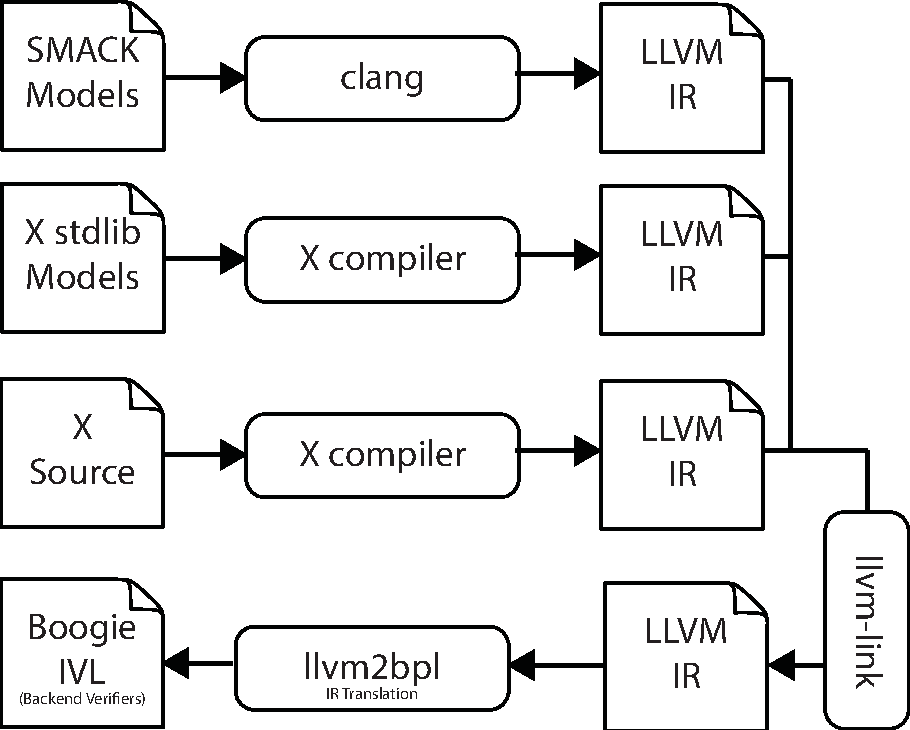
\includegraphics[width=\textwidth]{procedure}
% 	\caption{Toolflow for adding support for programming language X to SMACK.}
% 	\label{fig:vmcaixlang}
% \end{figure}

% \begin{table}[tb]
% \caption[List of programming languages we considered and their properties]{List of programming languages we considered and their properties.
%   Column \textbf{Ahead-of-Time} shows whether an Ahead-of-Time compiler
%   is available for the language;
%   %
%   column \textbf{LLVM 3.9} indicates whether the needed LLVM version is
%   supported;
%   %
%   column \textbf{Active} indicates whether the compiler is under active
%   development, while column \textbf{Stable} indicates if there is a
%   stable release;
%   %
%   and finally, column \textbf{Used it?} shows whether we used the language
%   in our evaluation.

% }
% \label{tab:languages}
% \centering
% \setlength{\tabcolsep}{6.5pt}
% \ra{2}
% \vspace{1em}
% \begin{tabular}{@{}lcccccc@{}}
% 	\toprule
% 	\textbf{Language} & \textbf{Compiler} & \textbf{Ahead-of-Time} & \textbf{LLVM 3.9} & \textbf{Active} & \textbf{Stable} & \textbf{Used it?} \\
% 	\midrule
% 	C & clang & \cmark & \cmark & \cmark & \cmark & \cmark \\
%         \hdashline[1pt/1pt]
% 	C++ & clang & \cmark & \cmark & \cmark & \cmark & \cmark \\
%         \hdashline[1pt/1pt]
% 	Fortran~\cite{flang-link} & flang & \cmark & \cmark & \cmark & \cmark & \cmark \\
%         \hdashline[1pt/1pt]
% 	D~\cite{d-link} & ldc & \cmark & \cmark & \cmark & \cmark & \cmark \\
%         \hdashline[1pt/1pt]
% 	Rust~\cite{rust-link} & rustc & \cmark & \cmark & \cmark & \cmark & \cmark \\
%         \hdashline[1pt/1pt]
% 	Objective-C & clang & \cmark & \cmark & \cmark & \cmark & \cmark \\
%         \hdashline[1pt/1pt]
% 	Swift~\cite{swift-link} & swiftc & \cmark & \cmark & \cmark & \cmark & \cmark \\
%         \hdashline[1pt/1pt]
% 	Kotlin~\cite{kotlin-link} & kotlinc & \cmark & \cmark & \cmark & \cmark & \cmark \\
%         \hdashline[1pt/1pt]
% 	Scala~\cite{scala-link} & scala-native & \cmark & \cmark & \cmark & \cmark & \xmark \\
%         \hdashline[1pt/1pt]
% 	C\#~\cite{llilc} & llilc & \cmark & ? & \cmark & \cmark & \xmark \\
%         \hdashline[1pt/1pt]
% 	Haskell~\cite{haskell-link} & ghc & \cmark & \cmark & \cmark & \cmark & \xmark \\
%         \hdashline[1pt/1pt]
% 	Julia~\cite{julia} & julia & \xmark & \cmark & \cmark & \xmark & \xmark \\
%         \hdashline[1pt/1pt]
% 	Go~\cite{go-link} & llgo & \cmark & \cmark & \xmark & \xmark & \xmark \\
%         \hdashline[1pt/1pt]
% 	Python~\cite{pyston-link} & pyston & \cmark & ? & \xmark & \xmark & \xmark \\
%         \hdashline[1pt/1pt]
% 	Ruby~\cite{ruby-link} & ruby-llvm & \cmark & \xmark & \xmark & \xmark & \xmark \\
%         \hdashline[1pt/1pt]
% 	Java~\cite{falcon-link} & falcon (Azul) & \xmark & \xmark & \cmark & \xmark & \xmark \\
% 	\bottomrule
% \end{tabular}
% \end{table}


% \begin{figure}[tb]
% 	\centering
% 	\begin{minipage}{.45\textwidth}
% \begin{lstlisting}[language=C,basicstyle=\ttfamily\large,commentstyle=\color{green},frame=lines,numberstyle=\tiny]
% int cap(int x) {
%   int y = x;
%   if (10 < x) {
%     y = 10;
%   }
%   return y;
% }

% int main(void) {
%   assert(cap(2)==2);
%   assert(cap(15)==10);
%   int x = nondet_int(); 
%   assert(cap(x) <= 10);
% }
% \end{lstlisting}
% 	\end{minipage}
% \hfill
% 	\begin{minipage}{.5\textwidth}
% \begin{lstlisting}[language=swift,basicstyle=\ttfamily\large,commentstyle=\color{green},frame=lines,numberstyle=\tiny]
% func cap(_ x: Int)->Int
% {
%   var y = x
%   if 10 < x {
%     y = 10
%   }
%   return y
% }

% assert(cap(2) == 2)
% assert(cap(15) == 10)
% let x=Int(nondet_int())
% assert(cap(x) <= 10)
% \end{lstlisting}    
%     \end{minipage}
% 	\begin{minipage}{.45\textwidth}
% \begin{lstlisting}[language=rust,basicstyle=\ttfamily\large,commentstyle=\color{green},frame=lines,numberstyle=\tiny]
% fn cap(x: usize)->usize
% {
%   let mut y = x;
%   if 10 < x {
%     y = 10;
%   }
%   return y;
% }


% fn main() {
%   let two = cap(2);
%   let ten = cap(15);
%   assert!(two == 2);
%   assert!(ten == 10);
%   let x = nondet_int();
%   assert!(x <= 10);
% }
% \end{lstlisting}
% 	\end{minipage}
% \hfill
% 	\begin{minipage}{.5\textwidth}
% \begin{lstlisting}[language=fortran,basicstyle=\ttfamily\large,commentstyle=\color{green},frame=lines,numberstyle=\tiny]
% pure function cap(x)
%  integer, intent(in)::x
%  integer :: cap, y
%  y = x
%  if (10 < y) then
%    y = 10
%  end if
%  cap = y
% end function

% program main
%  integer :: cap, x
%  call assert(cap(2)==2)
%  call assert(cap(15)==10)
%  x = nondet_int()
%  call assert(cap(x)<=10)
% end program main
% \end{lstlisting}    
%     \end{minipage}
% \caption{Microbenchmark with program versions in C, Swift, Rust, and Fortran.}
% \label{fig:microbenchmark}
% \end{figure}


% \begin{table}[tb]
% \caption[Characteristics of our microbenchmark suite]{Characteristics of our microbenchmark suite. Column \textbf{LOC} is the average
% number of lines of code per benchmark across supporting languages; column \textbf{\#Lang}
% is the number of languages supporting the features tested.}
% \vspace{1em}
% \label{tab:vmcaibenchmarks}
% \centering
% \setlength{\tabcolsep}{20pt}
% \ra{1.75}
% 	\begin{tabular}{@{}lcrr@{}}
% 	\toprule
% 	\textbf{Benchmark} & \textbf{Features Tested} & \textbf{LOC} & \textbf{\#Lang} \\
% 	\midrule
% 	basic    & basic assertions & 8 & 8 \\
%         \hdashline[1pt/1pt]
% 	compute  & integer arithmetic & 12 & 8 \\
%         \hdashline[1pt/1pt]
% 	function & functions, if-then-else, nondet values & 19 & 8 \\
%         \hdashline[1pt/1pt]
% 	forloop  & for loops & 14 & 8 \\
%         \hdashline[1pt/1pt]
% 	fib      & recursion & 20 & 8 \\
%         \hdashline[1pt/1pt]
% 	compound & objects and structures, fields & 18 & 8 \\
%         \hdashline[1pt/1pt]
% 	array    & array creation, array access & 10 & 8 \\
%         \hdashline[1pt/1pt]
% 	pointer  & dynamic memory allocation, references & 14 & 6 \\
%         \hdashline[1pt/1pt]
% 	inout    & updates via side effects & 17 & 7 \\
%         \hdashline[1pt/1pt]
% 	method   & single type dispatch & 26 & 6 \\
%         \hdashline[1pt/1pt]
% 	dynamic  & polymorphic dispatch & 29 & 6 \\
% 	\bottomrule
% \end{tabular}
% \end{table}

% \begin{table}[tb]
% \caption[Results of running SMACK on our microbenchmarks]{Results of running SMACK on our microbenchmarks. Symbol \cmark marks
% passing, symbol \xmark failing, and \notapplic marks benchmarks that do
% not have a version for the corresponding language.}
% \label{tab:results}
% \centering
% \setlength{\tabcolsep}{9pt}
% \vspace{1em}
% \ra{2}
% \begin{tabular}{@{}lcccccccc@{}}
% \toprule
% \textbf{Benchmark} & \textbf{C} & \textbf{C++} & \textbf{Objective-C} & \textbf{Rust} & \textbf{Fortran} & \textbf{D} & \textbf{Swift} & \textbf{Kotlin} \\
% \midrule
% basic & \cmark & \cmark & \cmark & \cmark & \cmark & \cmark & \cmark & \cmark \\
% \hdashline[1pt/1pt]
% compute & \cmark & \cmark & \cmark & \cmark & \cmark & \cmark & \cmark & \cmark \\
% \hdashline[1pt/1pt]
% function & \cmark & \cmark & \cmark & \cmark & \cmark & \cmark & \cmark & \cmark \\
% \hdashline[1pt/1pt]
% forloop & \cmark & \cmark & \cmark & \cmark & \cmark & \cmark & \xmark & \cmark \\
% \hdashline[1pt/1pt]
% fib & \cmark & \cmark & \cmark & \cmark & \cmark & \cmark & \cmark & \cmark \\
% \hdashline[1pt/1pt]
% compound & \cmark & \cmark & \xmark & \cmark & \cmark & \cmark & \cmark & \xmark \\
% \hdashline[1pt/1pt]
% array & \cmark & \cmark & \xmark & \cmark & \cmark & \cmark & \xmark & \xmark \\
% \hdashline[1pt/1pt]
% pointer & \cmark & \cmark & \cmark & \cmark & \cmark & \cmark & \notapplic & \notapplic \\
% \hdashline[1pt/1pt]
% inout & \cmark & \cmark & \cmark & \cmark & \cmark & \cmark & \cmark & \notapplic \\
% \hdashline[1pt/1pt]
% method & \notapplic & \cmark & \xmark & \cmark & \notapplic & \cmark & \xmark & \cmark \\
% \hdashline[1pt/1pt]
% dynamic & \notapplic & \xmark & \xmark & \cmark & \notapplic & \xmark & \xmark & \xmark \\
% \bottomrule
% \end{tabular}
% \end{table}

% \begin{table}[tb]
% \caption{Time commitment summary for adding a new language.}
% \label{tab:d-exercise}
% \centering
% \setlength{\tabcolsep}{10pt}
% \vspace{1em}
% \ra{1.75}
% \begin{tabular}{@{}lr@{}}
% 	\toprule
% 	\textbf{Procedure Step} & \textbf{Person-Hours} \\
% 	\midrule
% 	Write code to interoperate with SMACK models & 8 \\
% 	Compile and link at the LLVM-IR level, test  & 3 \\
% 	Add and model missing functionality          & 4 \\
%         \hdashline[1pt/1pt]
% 	\multicolumn{1}{r}{Total:}                 & 15 \\
% 	\bottomrule
% \end{tabular}
% \end{table}